\chapter{Cholesky Factorization Execution Time Analysis}
The \textbf{Cholesky decomposition algorithm} was first proposed by Andre-Louis \textbf{Cholesky} (October 15, 1875 - August 31, 1918) at the end of the First World War shortly before he was killed in battle. He was a French military officer and mathematician. The idea of this algorithm was published in 1924 by his fellow officer and, later, was used by Banachiewicz in 1938[2][3]. In the Russian mathematical literature, the Cholesky decomposition is also known as the square-root method due to the square root operations used in this decomposition and not used in Gaussian elimination.
\newline
Originally, the Cholesky decomposition was used only for dense real symmetric positive definite matrices. At present, the application of this decomposition is much wider. For example, it can also be employed for the case of Hermitian matrices. In order to increase the computing performance, its block versions are often applied.
\newline
In the case of sparse matrices, the Cholesky decomposition is also widely used as the main stage of a direct method for solving linear systems. In order to reduce the memory requirements and the profile of the matrix, special reordering strategies are applied to minimize the number of arithmetic operations. A number of reordering strategies are used to identify the independent matrix blocks for parallel computing systems.
%%%%% Introduction %%%%%%%%%
\section*{Introduction}
We investigate the execution times of the Cholesky decomposition procedure using MATLAB.The goal is to examine whether the execution times follow the cubic complexity predicted for $\Omega$ and to construct a corresponding mathematical function, $T_{\text{chol}}(n)$, using MATLAB's polyfit command.\newline

\subsection*{Source Code}
The following MATLAB code was used to measure the execution times, fit cubic polynomials, and compare predictions with actual timings.
% \newpage
\begin{center}
    \begin{lstlisting}[language=MATLAB, caption=Time Analysis Source Code]
    clc;
    clear all;
    %% Code Start form here
    %Measure  n = [100:100:2000]
    n_values = [100:100:2000];
    execution_times = zeros(size(n_values));
   
    for i = 1:length(n_values)
        
        A = randn(n_values(i));
        A = A * A'; 
        A = A + n_values(i) * eye(n_values(i)); 

        try
            timing = timeit(@() chol(A));
            execution_times(i) = timing;
        catch
            fprintf('Error for n = %d. Matrix is not positive definite.\n', n_values(i));
            execution_times(i) = NaN; 
        end
    end

    
    % Fit cubic polyfit
    degree = 3;
    [p, S, mu] = polyfit(n_values, execution_times, degree);

    %Predict results
    n_values_all = [100:100:2000];
    n_values_extra = [150:100:1550];

    predict_time = polyval(p, n_values_all, S, mu);
    predict_times_extra = polyval(p, n_values_extra, S, mu);

    figure;
    plot(n_values, execution_times, 'o','LineWidth', 1, 'MarkerSize', 8, 'Color', 'red', 'DisplayName', 'Measured Times');
    hold on;
    plot(n_values_all, predict_time, '-','LineWidth', 1, 'MarkerSize', 8, 'Color', 'green', 'DisplayName', 'Cubic Fit');

    % Add the predicted times for the extra values 
    plot(n_values_extra, predict_times_extra, 'x','LineWidth', 1, 'MarkerSize', 8, 'Color', 'blue', 'DisplayName', 'Predicted Times (Extra)');
    grid on;

    xlabel('Matrix Size ');
    ylabel('Execution Time ');
    title('Cholesky Decomposition Execution Time Analysis');
    legend('Location', 'SouthEast');

    % Trying polynomial degrees (2 and 4)
    plynomial_2 = 2;
    plynomial_4 = 4;

    [p_2, S_2, mu_2] = polyfit(n_values, execution_times, plynomial_2);
    [p_4, S_4, mu_4] = polyfit(n_values, execution_times, plynomial_4);

    predict_times_2 = polyval(p_2, n_values_all, S_2, mu_2);
    predict_times_4 = polyval(p_4, n_values_all, S_4, mu_4);

    %  results for degree 2 and degree 4
    figure;
    plot(n_values, execution_times, 'o', 'DisplayName', 'Measured Times');
    grid on;
    hold on;
    plot(n_values_all, predict_time, '-','LineWidth', 1, 'MarkerSize', 8, 'Color', 'red', 'DisplayName', 'Cubic Fit');
    plot(n_values_all, predict_times_2, '--','LineWidth', 1, 'MarkerSize', 8, 'Color', 'green', 'DisplayName', 'Degree 2 Fit');
    plot(n_values_all, predict_times_4, '-.','LineWidth', 1, 'MarkerSize', 8, 'Color','blue', 'DisplayName', 'Degree 4 Fit');

    xlabel('Matrix Size');
    ylabel('Execution Time');
    title('Cholesky Decomposition Execution Time Analysis with polynomial 2 and 4');
    legend('Location', 'SouthEast');

\end{lstlisting}
\end{center}
\newpage
%%%% Results %%%%%%%%%%
\section*{Results}
%%%% Cubic Polynomial Fit %%%%%%%%%
\subsection*{Cubic Polynomial Fit}
The execution times for matrix sizes $n = [100:100:2000]$ were measured, and a cubic polynomial fit was performed using MATLAB's \texttt{polyfit} command. The results are visualized in Figure \ref{fig:cubic_fit}.

\begin{figure}[ht]
    \centering
    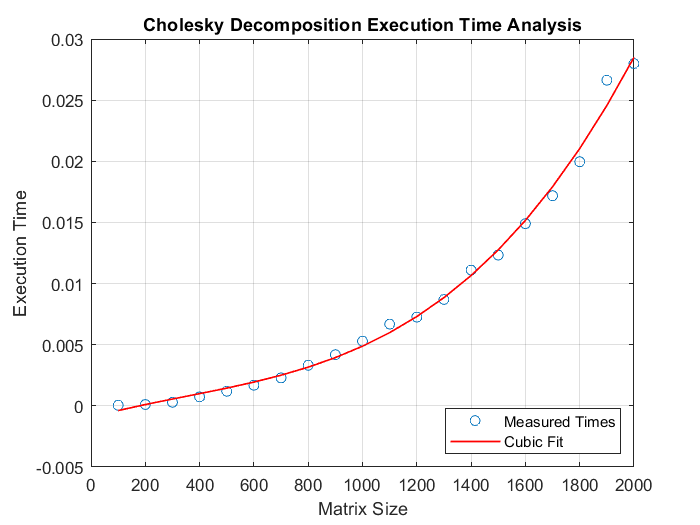
\includegraphics[width=0.8\textwidth]{Chapters/Predicted.png}
    \caption{Cubic Polynomial Fit for Cholesky Decomposition Execution Time}
    \label{fig:cubic_fit}
\end{figure}
The cubic polynomial fit precisely reflects the measured execution time complexity, demonstrating a cubic relationship with matrix size. This idea is critical for comprehending the computational behavior of Cholesky decomposition.

\newpage
%%%% Compatasion with predictions %%%%%%
\subsection*{Comparison with Predictions}

The predicted execution times for both the measured matrix sizes and additional values ($n = [150:100:1550]$) were calculated using the cubic polynomial function. The results are presented in Figure \ref{fig:prediction_comparison}.
\begin{figure}[ht]
    \centering
    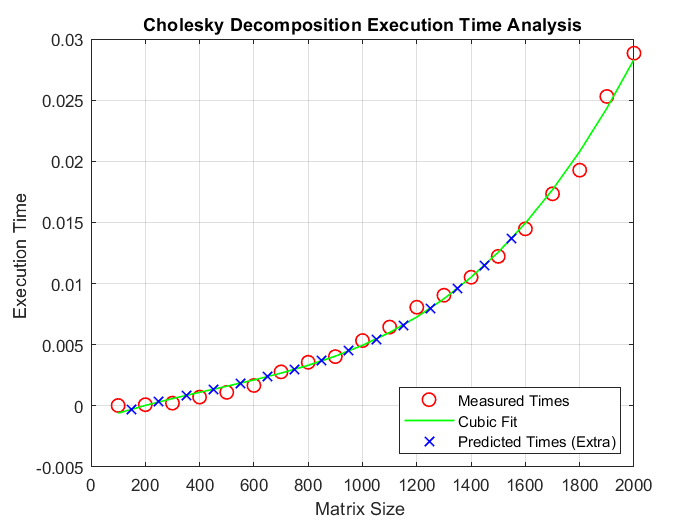
\includegraphics[width=0.8\textwidth]{Chapters/cholesky time analysis.png}
    \caption{Comparison of Measured and Predicted Execution Times}
    \label{fig:prediction_comparison}
\end{figure}
\newline
The figure shows the agreement between measured and anticipated values, demonstrating the cubic model's accuracy in capturing the Cholesky decomposition's execution time complexity.

\newpage
%%%%%%%% Deegree 2 and 4 poly fits %%%%%%%
\subsection*{Degree 2 and Degree 4 Polynomial Fits}

Additionally, polynomial fits of degrees 2 and 4 were performed to compare their predictions with the cubic polynomial. The results are shown in Figure \ref{fig:degree_comparison}.

\begin{figure}[ht]
    \centering
    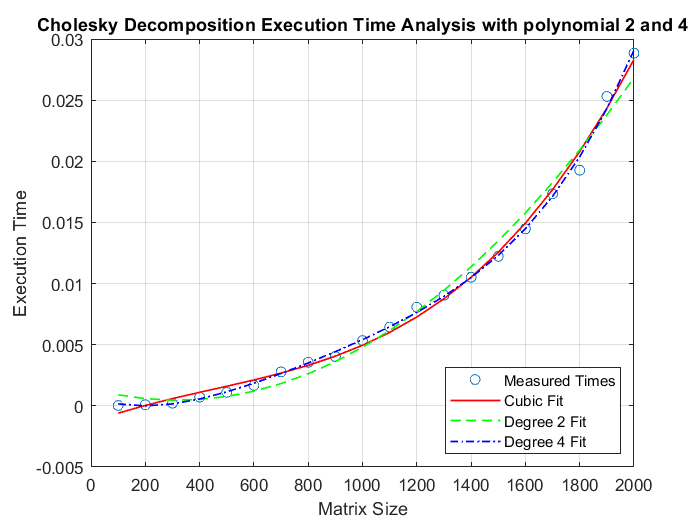
\includegraphics[width=0.8\textwidth]{Chapters/Time Analysis with poly 2,4.png}
    \caption{Comparison of Polynomial Fits (Degrees 2, 3, and 4)}
    \label{fig:degree_comparison}
\end{figure}
The figure demonstrates the significance of choosing an adequate polynomial degree for effective modeling. The cubic fit accurately represents the observed complexities, demonstrating its usefulness for capturing Cholesky decomposition execution time variations.
\section*{Conclusion}
In conclusion, this analysis sheds light on the execution times of the Cholesky decomposition operation, a fundamental operation in linear algebra and numerical computing. The cubic polynomial fit appears to accurately model the observed complexities, and comparisons with polynomial fits of degrees 2 and 4 highlight the cubic relationship. This investigation provides valuable insights for understanding the computational behavior of Cholesky decomposition and may have implications for optimizing algorithms or selecting appropriate computational resources.



